%%%%%%%%%%%%%%%%%%%%%%%%%%%%%%%%%%%%%%%%%%%%%%%%%%%%%%%%%%%%%%%%%%%%%%%%%%%%%%%
% CASE STUDY TEMPLATE - Programming and Problem Solving
% Author: Brendan Shea, PhD
% Course: Programming and Problem Solving
% Rochester Community and Technical College
%%%%%%%%%%%%%%%%%%%%%%%%%%%%%%%%%%%%%%%%%%%%%%%%%%%%%%%%%%%%%%%%%%%%%%%%%%%%%%%

\documentclass[11pt,letterpaper]{article}

%---------- PACKAGES ----------%
\usepackage[margin=1in, headheight=22pt]{geometry}
\usepackage[T1]{fontenc}
\usepackage{xcolor}
\usepackage{tcolorbox}
\usepackage{graphicx}
\usepackage{titlesec}
\usepackage{enumitem}
\usepackage{fancyhdr}
\usepackage{listings}
\usepackage{hyperref}
\usepackage{multicol}
\usepackage{booktabs}
\usepackage{tikz}
\usepackage{float}
\usepackage{amssymb}
\usepackage{amsmath}
\usepackage{pifont}

% TikZ libraries
\usetikzlibrary{shapes.geometric, arrows.meta, positioning, calc, backgrounds, fit, matrix, decorations.pathreplacing}

% Load tcolorbox libraries
\tcbuselibrary{skins,breakable,listings,listingsutf8}

%---------- COLOR DEFINITIONS ----------%
\definecolor{csprimary}{HTML}{2C3E50}
\definecolor{cssecondary}{HTML}{E74C3C}
\definecolor{cstertiary}{HTML}{3498DB}
\definecolor{csaccent}{HTML}{27AE60}
\definecolor{cswarm}{HTML}{F39C12}
\definecolor{cslight}{HTML}{ECF0F1}
\definecolor{csdark}{HTML}{1A252F}

% Syntax highlighting colors
\definecolor{codegreen}{HTML}{27AE60}
\definecolor{codepurple}{HTML}{9B59B6}
\definecolor{codeorange}{HTML}{E67E22}
\definecolor{codeblue}{HTML}{3498DB}
\definecolor{codegray}{HTML}{95A5A6}
\definecolor{codestring}{HTML}{E74C3C}
\definecolor{codebg}{HTML}{1E2A38}

%---------- CASE STUDY METADATA ----------%
\newcommand{\cstitle}{Objects All the Way Down}
\newcommand{\cssubtitle}{The History and Philosophy of Object-Oriented Programming}
\newcommand{\csauthor}{Brendan Shea, PhD}
\newcommand{\cscourse}{Programming and Problem Solving}
\newcommand{\csinstitution}{Rochester Community and Technical College}
\newcommand{\csdate}{\today}

%---------- LISTINGS CONFIGURATION ----------%
\lstdefinestyle{basestyle}{
    backgroundcolor=\color{codebg},
    basicstyle=\ttfamily\small\color{white},
    breakatwhitespace=false,
    breaklines=true,
    captionpos=b,
    keepspaces=true,
    showspaces=false,
    showstringspaces=false,
    showtabs=false,
    tabsize=4,
    frame=none,
    xleftmargin=4mm,
    xrightmargin=4mm,
    aboveskip=0pt,
    belowskip=0pt,
}

\lstdefinestyle{javastyle}{
    style=basestyle,
    language=Java,
    keywordstyle=\color{codeblue}\bfseries,
    commentstyle=\color{codegray}\itshape,
    stringstyle=\color{codestring},
    morekeywords={String, Scanner, System, var, boolean, record, sealed, permits, yield},
}

\lstdefinestyle{simulastyle}{
    style=basestyle,
    keywordstyle=\color{codeblue}\bfseries,
    commentstyle=\color{codegray}\itshape,
    morekeywords={BEGIN, END, CLASS, REF, NEW, THIS, VIRTUAL, INTEGER, REAL, BOOLEAN, TEXT, PROCEDURE},
}

\lstdefinestyle{smalltalkstyle}{
    style=basestyle,
    keywordstyle=\color{codeblue}\bfseries,
    commentstyle=\color{codegray}\itshape,
    morekeywords={self, super, true, false, nil, ifTrue, ifFalse, whileTrue, new},
}

%---------- CUSTOM ENVIRONMENTS ----------%
\newcommand{\keyterm}[1]{\textbf{\textcolor{cssecondary}{#1}}}

\newtcolorbox{conceptbox}[1][]{
    enhanced,
    colback=cslight,
    colframe=csprimary,
    fonttitle=\bfseries\color{white},
    title=#1,
    attach boxed title to top left={yshift=-2mm, xshift=5mm},
    boxed title style={colback=csprimary},
    breakable
}

\newtcolorbox{historybox}[1][]{
    enhanced,
    colback=codepurple!8,
    colframe=codepurple,
    fonttitle=\bfseries\color{white},
    title=#1,
    attach boxed title to top left={yshift=-2mm, xshift=5mm},
    boxed title style={colback=codepurple},
    breakable
}

\newtcolorbox{debatebox}[1][]{
    enhanced,
    colback=cswarm!8,
    colframe=cswarm,
    fonttitle=\bfseries\color{white},
    title=#1,
    attach boxed title to top left={yshift=-2mm, xshift=5mm},
    boxed title style={colback=cswarm},
    breakable
}

\newtcolorbox{quotebox}[1][]{
    enhanced,
    colback=cstertiary!8,
    colframe=cstertiary,
    fonttitle=\bfseries\color{white},
    title=#1,
    attach boxed title to top left={yshift=-2mm, xshift=5mm},
    boxed title style={colback=cstertiary},
    breakable
}

\newtcblisting{javacode}[1][]{
    enhanced,
    colback=codebg,
    colframe=csaccent,
    colupper=white,
    fonttitle=\bfseries\color{white},
    title=#1,
    attach boxed title to top left={yshift=-2mm, xshift=5mm},
    boxed title style={colback=csaccent},
    left=0mm, right=0mm, top=2mm, bottom=2mm,
    boxrule=1pt,
    breakable,
    pad at break=2mm,
    listing only,
    listing options={style=javastyle}
}

\newtcblisting{simulacode}[1][]{
    enhanced,
    colback=codebg,
    colframe=codepurple,
    colupper=white,
    fonttitle=\bfseries\color{white},
    title=#1,
    attach boxed title to top left={yshift=-2mm, xshift=5mm},
    boxed title style={colback=codepurple},
    left=0mm, right=0mm, top=2mm, bottom=2mm,
    boxrule=1pt,
    breakable,
    pad at break=2mm,
    listing only,
    listing options={style=simulastyle}
}

\newtcblisting{smalltalkcode}[1][]{
    enhanced,
    colback=codebg,
    colframe=cstertiary,
    colupper=white,
    fonttitle=\bfseries\color{white},
    title=#1,
    attach boxed title to top left={yshift=-2mm, xshift=5mm},
    boxed title style={colback=cstertiary},
    left=0mm, right=0mm, top=2mm, bottom=2mm,
    boxrule=1pt,
    breakable,
    pad at break=2mm,
    listing only,
    listing options={style=smalltalkstyle}
}

\newtcolorbox{questionbox}{
    enhanced,
    colback=cswarm!10,
    colframe=cswarm,
    fonttitle=\bfseries\color{white},
    title=Discussion Questions,
    attach boxed title to top center={yshift=-2mm},
    boxed title style={colback=cswarm},
    breakable
}

\newtcolorbox{glossarybox}{
    enhanced,
    colback=cslight,
    colframe=csprimary,
    fonttitle=\bfseries\color{white},
    title=Glossary of Key Terms,
    attach boxed title to top center={yshift=-2mm},
    boxed title style={colback=csprimary},
    breakable
}

%---------- HEADER/FOOTER ----------%
\pagestyle{fancy}
\fancyhf{}
\fancyhead[L]{\small\textcolor{csprimary}{\cscourse}}
\fancyhead[R]{\small\textcolor{csprimary}{Case Study}}
\fancyfoot[C]{\thepage}
\renewcommand{\headrulewidth}{0.4pt}
\renewcommand{\headrule}{\hbox to\headwidth{\color{csprimary}\leaders\hrule height \headrulewidth\hfill}}

%---------- SECTION FORMATTING ----------%
\titleformat{\section}
    {\Large\bfseries\color{csprimary}}
    {\thesection}{1em}{}[\color{cssecondary}\titlerule]
    
\titleformat{\subsection}
    {\large\bfseries\color{cstertiary}}
    {\thesubsection}{1em}{}

%---------- HYPERLINK SETTINGS ----------%
\hypersetup{
    colorlinks=true,
    linkcolor=cstertiary,
    urlcolor=cstertiary
}

%%%%%%%%%%%%%%%%%%%%%%%%%%%%%%%%%%%%%%%%%%%%%%%%%%%%%%%%%%%%%%%%%%%%%%%%%%%%%%%
\begin{document}

%---------- TITLE BLOCK ----------%
\begin{tcolorbox}[
    enhanced,
    colback=csprimary,
    colframe=csprimary,
    arc=0mm,
    left=10mm, right=10mm, top=8mm, bottom=8mm
]
\begin{center}
    {\huge\bfseries\color{white}\cstitle}\\[3mm]
    {\Large\color{cslight}\cssubtitle}\\[5mm]
    \textcolor{cssecondary}{\rule{0.5\textwidth}{1pt}}\\[5mm]
    {\large\color{white}\csauthor}\\[2mm]
    {\normalsize\color{cslight}\cscourse\ $\bullet$ \csinstitution}
\end{center}
\end{tcolorbox}

\vspace{5mm}

%---------- INTRODUCTION ----------%
\section*{Introduction}

When you write \texttt{String greeting = "Hello"} in Java, you're participating in a philosophy of programming that has shaped software development for over fifty years. That \texttt{String} isn't just data---it's an \keyterm{object}: a bundle of data and behavior, a little machine that knows how to do things like report its length, convert to uppercase, or find substrings within itself.

\keyterm{Object-oriented programming} (OOP) is so dominant today that it can seem like the natural, obvious way to write software. But OOP is a human invention with a specific history, created by specific people trying to solve specific problems. Understanding that history illuminates not just how to use objects, but \textit{why} they exist, what problems they solve, and what tradeoffs they embody.

This case study traces OOP from its origins in 1960s Norway through its explosive growth in the 1990s to ongoing debates about its future. Along the way, you'll meet the visionaries who shaped how we think about software, explore the philosophical ideas underlying OOP, and examine how modern languages like Java continue to evolve.

\begin{conceptbox}[The Central Metaphor]
Object-oriented programming asks us to think about software as a collection of \textbf{objects}---independent entities that have their own data (state) and their own behaviors (methods). Objects interact by sending messages to each other, much like people or organizations in the real world.

This metaphor is powerful but not inevitable. Other paradigms organize code around functions, logic rules, or data transformations. OOP's dominance reflects both its genuine strengths and historical contingency.
\end{conceptbox}

%---------- THE PROBLEM OF COMPLEXITY ----------%
\section{The Problem of Complexity}

To understand why OOP emerged, we must first understand what problems it was trying to solve.

By the 1960s, software was growing increasingly complex. Programs that had once fit in a few hundred lines now sprawled across thousands. Teams of programmers needed to collaborate on single systems. And the \keyterm{software crisis} loomed: projects ran over budget, delivered late, and failed to meet requirements. The tools and techniques that worked for small programs didn't scale.

The fundamental challenge was \keyterm{managing complexity}. How do you organize a program with 100,000 lines of code so that humans can understand it? How do you divide work among programmers so they don't constantly interfere with each other? How do you change one part of a system without breaking everything else?

\begin{historybox}[The Software Crisis]
At the 1968 NATO Software Engineering Conference, participants coined the term ``software crisis'' to describe the state of the industry. Software projects routinely failed. The IBM OS/360 operating system, one of the largest software projects of its era, ran years late and millions over budget. Project manager Fred Brooks later wrote \textit{The Mythical Man-Month}, observing that adding programmers to a late project makes it later---because communication overhead grows faster than productivity.

The conference concluded that software development needed to become more like engineering: disciplined, methodical, and based on sound principles. The search was on for better ways to structure programs.
\end{historybox}

%---------- SIMULA: THE BIRTH OF OBJECTS ----------%
\section{Simula: The Birth of Objects}

The first object-oriented language emerged not from the software crisis directly, but from an unexpected domain: simulation.

\begin{historybox}[Kristen Nygaard and Ole-Johan Dahl (1960s)]
At the Norwegian Computing Center in Oslo, Kristen Nygaard and Ole-Johan Dahl were working on simulation problems: modeling ships in harbors, customers in banks, traffic in cities. They realized that simulation naturally involves \textit{entities} with their own properties and behaviors---a ship has a position and speed; it can dock, load cargo, and depart.

In 1962, they began developing \textbf{Simula}, a language designed around this insight. By 1967, Simula 67 introduced the key concepts we now associate with OOP: classes, objects, inheritance, and polymorphism. Nygaard and Dahl had invented object-oriented programming---though the term wouldn't be coined until later.

Their work earned them the 2001 Turing Award, computing's highest honor. Sadly, both died in 2002, just months after receiving it.
\end{historybox}

Simula introduced the \keyterm{class}: a template or blueprint defining what data an object contains and what operations it can perform. You could define a \texttt{Ship} class once, then create many individual ship objects from it.

\begin{simulacode}[Simula 67: An Early Class]
CLASS Ship;
BEGIN
    INTEGER length, cargo;
    REAL speed;
    
    PROCEDURE dock;
    BEGIN
        speed := 0;
        ! Ship stops when docked
    END;
    
    PROCEDURE loadCargo(amount);
    INTEGER amount;
    BEGIN
        cargo := cargo + amount;
    END;
END;
\end{simulacode}

Simula also introduced \keyterm{inheritance}: a new class could be defined as an extension of an existing one, inheriting its data and behavior while adding or modifying features. A \texttt{CargoShip} could inherit from \texttt{Ship}, adding cargo-specific capabilities.

The key insight was that simulation's need to model real-world entities was actually a general programming need. The same techniques that helped simulate ships could help build any complex system.

%---------- SMALLTALK: THE VISION CRYSTALLIZES ----------%
\section{Smalltalk: Objects as Philosophy}

If Simula invented the mechanisms of OOP, \textbf{Smalltalk} articulated its philosophy. Developed at Xerox PARC in the 1970s under the leadership of Alan Kay, Smalltalk pursued the object metaphor to its logical extreme.

\begin{historybox}[Alan Kay and the Dynabook Dream]
Alan Kay joined Xerox PARC with a radical vision: the \textbf{Dynabook}, a portable computer for children that would revolutionize education and creativity. Though the hardware wasn't yet feasible, Kay's team built the software environment it would need: Smalltalk.

Kay was influenced by biology (cells as independent units), mathematics (Lisp's elegant uniformity), and educational psychology (children's learning styles). He wanted a system where everything---numbers, windows, even the programming environment itself---was an object that could be inspected, modified, and combined.

Kay is often credited with coining ``object-oriented,'' though he later said the term led people astray. He emphasized \textit{messaging}---objects communicating---over classes and inheritance. ``I made up the term object-oriented,'' he wrote, ``and I can tell you I did not have C++ in mind.''
\end{historybox}

Smalltalk embodied a purer vision of OOP than most languages that followed:

\begin{quotebox}[Alan Kay on Objects]
``I thought of objects being like biological cells and/or individual computers on a network, only able to communicate with messages... OOP to me means only messaging, local retention and protection and hiding of state-process, and extreme late-binding of all things.''
\end{quotebox}

In Smalltalk, \textit{everything} is an object---including numbers, booleans, and classes themselves. Even control flow works through message-passing: the boolean \texttt{true} responds to an \texttt{ifTrue:} message by executing the associated block.

\begin{smalltalkcode}[Smalltalk: Everything is an Object]
"Even integers are objects that receive messages"
3 + 4           "sends + message to 3 with argument 4"
'hello' size    "sends size message to string"

"Conditionals are messages to booleans"
(x > 0) ifTrue: [Transcript show: 'positive']
        ifFalse: [Transcript show: 'non-positive']

"Creating objects"
ship := Ship new.
ship loadCargo: 50.
\end{smalltalkcode}

Smalltalk also pioneered the graphical programming environment: windows, menus, and a mouse-driven interface---technologies that Xerox PARC developed and Apple later commercialized. The Smalltalk IDE allowed programmers to inspect and modify running objects, blurring the line between programming and using software.

%---------- THE OOP EXPLOSION ----------%
\section{The OOP Explosion: C++ and Java}

Simula and Smalltalk were influential but not widely adopted in mainstream industry. That changed in the 1980s and 1990s as OOP went from academic curiosity to industry standard.

\begin{historybox}[Bjarne Stroustrup and C++ (1979--)]
Bjarne Stroustrup, a Danish computer scientist at Bell Labs, wanted to combine the efficiency of C with the organizational power of Simula. Starting in 1979, he developed ``C with Classes,'' which evolved into \textbf{C++} by 1983.

C++ made a pragmatic choice: rather than pursuing object purity like Smalltalk, it added OOP features to a language programmers already knew. You could write C-style code where needed for performance, and use objects where they helped organization. This ``multi-paradigm'' approach---OOP without dogma---proved enormously appealing.

By the 1990s, C++ dominated systems programming, games, and applications requiring high performance. Its influence shaped a generation of languages.
\end{historybox}

\begin{historybox}[James Gosling and Java (1991--1995)]
At Sun Microsystems, James Gosling led a team developing software for interactive television. The project failed commercially, but produced a new language: \textbf{Java}.

Java took lessons from C++ (and its pain points): automatic memory management eliminated whole categories of bugs; a simpler object model avoided C++'s complexity; and compilation to bytecode running on a virtual machine enabled ``write once, run anywhere'' portability.

Java launched publicly in 1995, riding the wave of the early web (Java applets could run in browsers). By the 2000s, it dominated enterprise software development. Its influence extended to C\#, Kotlin, and countless other languages.
\end{historybox}

Java struck a balance between Smalltalk's object purity and C++'s pragmatism. Almost everything is an object (except primitives like \texttt{int} and \texttt{boolean}), but the language provides familiar control structures rather than message-passing for conditionals and loops.

%---------- THE PHILOSOPHY OF OOP ----------%
\section{The Philosophy: Modeling the World}

What makes OOP philosophically distinctive? Several interconnected ideas:

\subsection{Objects as Models}

OOP encourages thinking of programs as \keyterm{models} of some domain. A banking system has \texttt{Account}, \texttt{Customer}, and \texttt{Transaction} objects because banks have accounts, customers, and transactions. The code mirrors the conceptual structure of what it represents.

\begin{center}
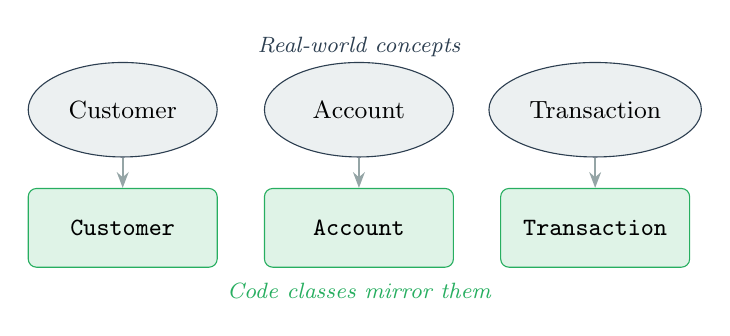
\begin{tikzpicture}[
    concept/.style={ellipse, draw=csprimary, fill=cslight, minimum width=24mm, minimum height=12mm, font=\small},
    code/.style={rectangle, rounded corners=3pt, draw=csaccent, fill=csaccent!15, minimum width=24mm, minimum height=10mm, font=\small\ttfamily},
    arrow/.style={-{Stealth[length=2mm]}, thick, color=codegray}
]

% Real world concepts
\node[concept] (cust) at (0,1.5) {Customer};
\node[concept] (acct) at (3,1.5) {Account};
\node[concept] (trans) at (6,1.5) {Transaction};

% Code classes
\node[code] (custc) at (0,0) {Customer};
\node[code] (acctc) at (3,0) {Account};
\node[code] (transc) at (6,0) {Transaction};

% Arrows
\draw[arrow] (cust) -- (custc);
\draw[arrow] (acct) -- (acctc);
\draw[arrow] (trans) -- (transc);

% Labels
\node[font=\footnotesize\itshape, color=csprimary] at (3,2.3) {Real-world concepts};
\node[font=\footnotesize\itshape, color=csaccent] at (3,-0.8) {Code classes mirror them};

\end{tikzpicture}
\end{center}

This modeling perspective makes OOP intuitive for many domains. But it also raises questions: How do we model concepts that don't have real-world counterparts? Is the ``real world'' really made of objects, or is that just one way of seeing it?

\subsection{Encapsulation: Hiding Complexity}

\keyterm{Encapsulation} means bundling data with the operations that manipulate it, and hiding internal details behind a public interface. A \texttt{BankAccount} object manages its own balance; other code interacts only through methods like \texttt{deposit()} and \texttt{withdraw()}, never touching the balance directly.

\begin{javacode}[Encapsulation in Java]
public class BankAccount {
    private double balance;  // Hidden from outside
    
    public void deposit(double amount) {
        if (amount > 0) {
            balance += amount;
        }
    }
    
    public boolean withdraw(double amount) {
        if (amount > 0 && amount <= balance) {
            balance -= amount;
            return true;
        }
        return false;  // Withdrawal failed
    }
    
    public double getBalance() {
        return balance;  // Controlled access
    }
}
\end{javacode}

Encapsulation enables \keyterm{information hiding}: you can change how a class works internally without affecting code that uses it. As long as the public interface stays stable, the implementation can evolve freely.

\subsection{Inheritance: Sharing and Specializing}

\keyterm{Inheritance} allows new classes to be defined as extensions of existing ones. A \texttt{SavingsAccount} can inherit from \texttt{BankAccount}, gaining all its capabilities while adding interest calculation.

\begin{javacode}[Inheritance: Extending a Class]
public class SavingsAccount extends BankAccount {
    private double interestRate;
    
    public SavingsAccount(double rate) {
        this.interestRate = rate;
    }
    
    public void applyInterest() {
        double interest = getBalance() * interestRate;
        deposit(interest);
    }
}
\end{javacode}

Inheritance creates an ``is-a'' relationship: a \texttt{SavingsAccount} \textit{is a} \texttt{BankAccount}. Anywhere a \texttt{BankAccount} is expected, a \texttt{SavingsAccount} can be used.

\subsection{Polymorphism: Many Forms}

\keyterm{Polymorphism} (from Greek: ``many forms'') means that code can work with objects of different types through a common interface. A method that accepts a \texttt{BankAccount} can work with any subclass---\texttt{SavingsAccount}, \texttt{CheckingAccount}, or types not yet invented.

\begin{javacode}[Polymorphism in Action]
public void printStatement(BankAccount account) {
    // Works with ANY kind of BankAccount
    System.out.println("Balance: $" + account.getBalance());
}

// Can be called with different types
printStatement(new SavingsAccount(0.02));
printStatement(new CheckingAccount());
\end{javacode}

Polymorphism enables extensibility: new types can be added without modifying existing code that works with the parent type.

%---------- CRITIQUES AND DEBATES ----------%
\section{Critiques and Ongoing Debates}

OOP's dominance hasn't gone unchallenged. Several critiques have emerged over decades of experience.

\begin{debatebox}[Inheritance: Blessing or Curse?]
Inheritance seemed like a great idea: define common behavior once, specialize where needed. In practice, deep inheritance hierarchies often became fragile and confusing. Changing a base class could break subclasses in unexpected ways (the ``fragile base class problem'').

Many experienced developers now advise: \textbf{``Favor composition over inheritance.''} Instead of making \texttt{SavingsAccount} inherit from \texttt{BankAccount}, have it \textit{contain} a \texttt{BankAccount} and delegate to it. This is more flexible but more verbose.

Java's designers have moved in this direction: default methods on interfaces, records, and sealed classes provide alternatives to classical inheritance hierarchies.
\end{debatebox}

\begin{debatebox}[Objects vs.\ Functions]
\keyterm{Functional programming}---organizing code around pure functions and immutable data---offers a different paradigm. Functional advocates argue that OOP's mutable objects make programs harder to reason about, especially in concurrent systems. When objects can change state, tracking what happened when becomes difficult.

The debate isn't binary. Modern languages increasingly blend paradigms: Java added lambdas and streams; functional languages like Scala include objects. Perhaps the question isn't ``which is better?'' but ``which is better for what?''
\end{debatebox}

\begin{debatebox}[Does OOP Model Reality?]
OOP claims to model the real world, but critics argue this is misleading. The world doesn't obviously consist of discrete objects with clear boundaries. A ``customer'' in code might correspond to a database record, a legal entity, a biological person, or a social role---all different things with different behaviors.

Moreover, some problems don't fit the object model well. Mathematical computations, data transformations, and event-driven systems may be more naturally expressed in other paradigms.
\end{debatebox}

%---------- MODERN DEVELOPMENTS ----------%
\section{Modern Developments: Java Evolves}

Java hasn't stood still. Recent versions have introduced features that respond to decades of OOP experience---and borrow ideas from other paradigms.

\subsection{Records: Data Without Boilerplate}

Sometimes you just want a class that holds data. Traditional Java required writing constructors, getters, \texttt{equals()}, \texttt{hashCode()}, and \texttt{toString()}---tedious boilerplate. \keyterm{Records} (Java 14+) generate all of this automatically:

\begin{javacode}[Records: Concise Data Classes (Java 14+)]
// Old way: ~30 lines of boilerplate
public class Point {
    private final int x;
    private final int y;
    public Point(int x, int y) { this.x = x; this.y = y; }
    public int getX() { return x; }
    public int getY() { return y; }
    // Plus equals(), hashCode(), toString()...
}

// New way: one line
public record Point(int x, int y) { }

// Usage is identical
Point p = new Point(3, 4);
System.out.println(p.x());  // 3
\end{javacode}

Records are immutable by default---a nod toward functional programming's emphasis on unchanging data.

\subsection{Sealed Classes: Controlled Inheritance}

Traditional inheritance is open: anyone can extend your class. \keyterm{Sealed classes} (Java 17) let you specify exactly which classes can extend yours:

\begin{javacode}[Sealed Classes: Controlled Hierarchies (Java 17)]
public sealed class Shape 
    permits Circle, Rectangle, Triangle {
    // Only these three can extend Shape
}

public final class Circle extends Shape {
    private double radius;
    // ...
}

public final class Rectangle extends Shape {
    private double width, height;
    // ...
}
\end{javacode}

This enables exhaustive pattern matching: the compiler can verify you've handled all cases.

\subsection{Pattern Matching: Smarter Conditionals}

\keyterm{Pattern matching} (Java 16+) lets you test an object's type and extract data in one step:

\begin{javacode}[Pattern Matching (Java 16+)]
// Old way: instanceof then cast
if (obj instanceof String) {
    String s = (String) obj;
    System.out.println(s.length());
}

// New way: pattern matching
if (obj instanceof String s) {
    System.out.println(s.length());  // s already available
}

// Switch expressions with patterns (Java 21)
String description = switch (shape) {
    case Circle c    -> "Circle with radius " + c.radius();
    case Rectangle r -> "Rectangle " + r.width() + "x" + r.height();
    case Triangle t  -> "Triangle";
};
\end{javacode}

\subsection{Functional Features}

Java 8 introduced \keyterm{lambdas} and the \keyterm{Stream API}, bringing functional programming into the object-oriented world:

\begin{javacode}[Functional Programming in Java]
List<String> names = List.of("Alice", "Bob", "Charlie");

// Lambda expression
names.forEach(name -> System.out.println(name));

// Stream pipeline: filter, transform, collect
List<String> longNames = names.stream()
    .filter(name -> name.length() > 4)
    .map(String::toUpperCase)
    .toList();
// Result: ["ALICE", "CHARLIE"]
\end{javacode}

These features don't replace OOP but complement it. Modern Java is increasingly multi-paradigm.

%---------- BEYOND JAVA ----------%
\section{Beyond Java: The Landscape Today}

Java's influence extends to newer languages that refine its ideas:

\textbf{Kotlin} (JetBrains, 2011) runs on the JVM but with more concise syntax, null safety built into the type system, and first-class support for functional programming. It's now Google's preferred language for Android development.

\textbf{Scala} (Martin Odersky, 2004) blends OOP and functional programming more deeply, with powerful type inference and pattern matching. It's popular for big data processing (Apache Spark).

\textbf{Swift} (Apple, 2014) and \textbf{Rust} (Mozilla, 2010) take different approaches to OOP: Swift uses protocols (like interfaces) rather than inheritance; Rust doesn't have inheritance at all, relying on traits and composition.

The trend is toward \textbf{multi-paradigm} languages that support objects when useful but don't force everything into the object mold.

%---------- CONCLUSION ----------%
\section{The Ongoing Conversation}

Object-oriented programming emerged from specific historical circumstances: the software crisis, simulation research, visions of personal computing. Its success reshaped the industry, but its core ideas remain contested and evolving.

Some questions for reflection: Is OOP's dominance deserved, or partly historical accident? Would a world that had bet on functional programming look very different? As AI increasingly writes code, does the paradigm that helps \textit{humans} organize programs even matter?

These aren't questions with settled answers. The history of programming is still being written---and you're now part of it.

%---------- DISCUSSION QUESTIONS ----------%
\section*{Discussion Questions}

\begin{questionbox}
\begin{enumerate}[leftmargin=*, label=\textcolor{cswarm}{\textbf{\arabic*.}}]
    \item \textbf{Modeling Reality:} OOP encourages modeling programs after real-world entities. But the ``real world'' can be carved up in many ways---there's no single right set of objects. How do programmers decide what objects to create? Is this a technical decision, a design decision, or something else?

    \item \textbf{Inheritance Reconsidered:} Early OOP emphasized inheritance as a key benefit. Modern practice often prefers composition. What went wrong with inheritance? Are there cases where it's still the right choice? How do newer features like records and sealed classes change the calculus?

    \item \textbf{Paradigm Wars:} Object-oriented and functional programming represent different philosophies. Is one ``better,'' or are they suited to different problems? What might a program look like that uses both approaches effectively?

    \item \textbf{Historical Contingency:} OOP's dominance owes much to historical factors: C++'s compatibility with C, Java's timing with the web, corporate backing, university curricula. If history had gone differently---if Smalltalk or Lisp had become mainstream---how might software development be different today?

    \item \textbf{The Future of OOP:} Languages keep evolving, blending paradigms, and adding features. Will ``object-oriented programming'' still be a meaningful category in 20 years? What might replace or transform it?
\end{enumerate}
\end{questionbox}

%---------- GLOSSARY ----------%
\section*{Key Terms}

\begin{glossarybox}
\begin{description}[leftmargin=!, labelwidth=3.2cm, font=\bfseries\color{cssecondary}]
    \item[Class] A blueprint or template defining the data and behavior that objects of that type will have.
    
    \item[Composition] Building complex objects by combining simpler ones, often preferred over inheritance for flexibility.
    
    \item[Encapsulation] Bundling data with methods that operate on it, hiding internal details behind a public interface.
    
    \item[Functional Programming] A paradigm organizing code around pure functions and immutable data, contrasting with OOP's mutable objects.
    
    \item[Inheritance] A mechanism where new classes are defined as extensions of existing ones, inheriting their data and behavior.
    
    \item[Lambda] An anonymous function that can be passed as a value, enabling functional programming patterns.
    
    \item[Object] An instance of a class, combining state (data) and behavior (methods) into a single entity.
    
    \item[Pattern Matching] A feature allowing code to test an object's type and extract its data simultaneously.
    
    \item[Polymorphism] The ability to treat objects of different types uniformly through a common interface.
    
    \item[Record] A concise way to declare classes that are primarily data carriers, with automatically generated boilerplate.
    
    \item[Sealed Class] A class that specifies exactly which other classes may extend it, enabling exhaustive handling.
    
    \item[Stream API] Java's library for functional-style operations on collections, using pipelines of filter, map, and reduce.
\end{description}
\end{glossarybox}

\vspace{5mm}

%---------- FOOTER ----------%
\begin{center}
\textcolor{csprimary}{\rule{0.6\textwidth}{0.5pt}}\\[3mm]
{\small\textcolor{gray}{This case study is part of the Open Educational Resources for \cscourse.\\
Licensed under Creative Commons Attribution 4.0 (CC BY 4.0).}}
\end{center}

\end{document}
